% Model development and optimization, hyper-parameter tuning, cross-validation, evaluation of models
\section{Models}

\subsection{Logistic Regression}
To develop the logistic regression model, we used the scikit-learn library in Python. The dataset was preprocessed by selecting 13 key features and converting the multi-class target variable $(1 - 4)$ into a binary target for heart disease classification. Missing values were handled using mean imputation, and we normalized the feature values using min-max scaling to ensure all features were on a similar scale.

The Logistic Regression model inherently uses the sigmoid activation function to model the probability of the target class (disease or no disease). The sigmoid function transforms the linear combination of the input features, $z = w^{T}X + b$ (where \(w\) represents the weights and \(b\) the bias), into a probability value between 0 and 1. This transformation is defined as:

\[
P(y=1 \mid X) = \frac{1}{1 + e^{-z}}
\]

The dataset was split into 75\% training and 25\% testing sets using the binary cross-entropy loss function which measures the difference between the predicted probabilities and the actual target labels. When making predictions, the model assigns the class label based on a threshold of 0.5, where: 
If $\textnormal{P}(y=1 \mid X) \geq 0.5$,  the prediction is "Disease".
If $\textnormal{P}(y=1 \mid X) < 0.5$, the prediction is "No Disease".

The initial model, trained without hyperparameter tuning or cross-validation, achieved a precision of 0.86, accuracy of 0.89, recall of 0.86, specificity of 0.87, and an F1-Score of 0.86, indicating balanced performance for the task. After applying cross-validation and hyperparameter tuning, the updated model achieved improved metrics: precision of 0.89, accuracy of 0.83, recall of 0.86, specificity of 0.90, and an F1-Score of 0.88. (Fig.~\ref{Initial Logistic Regression Confusion Matrix} \& Fig.~\ref{Tuned Logistic Regression Confusion Matrix})

\begin{figure}[htbp]
    \centerline{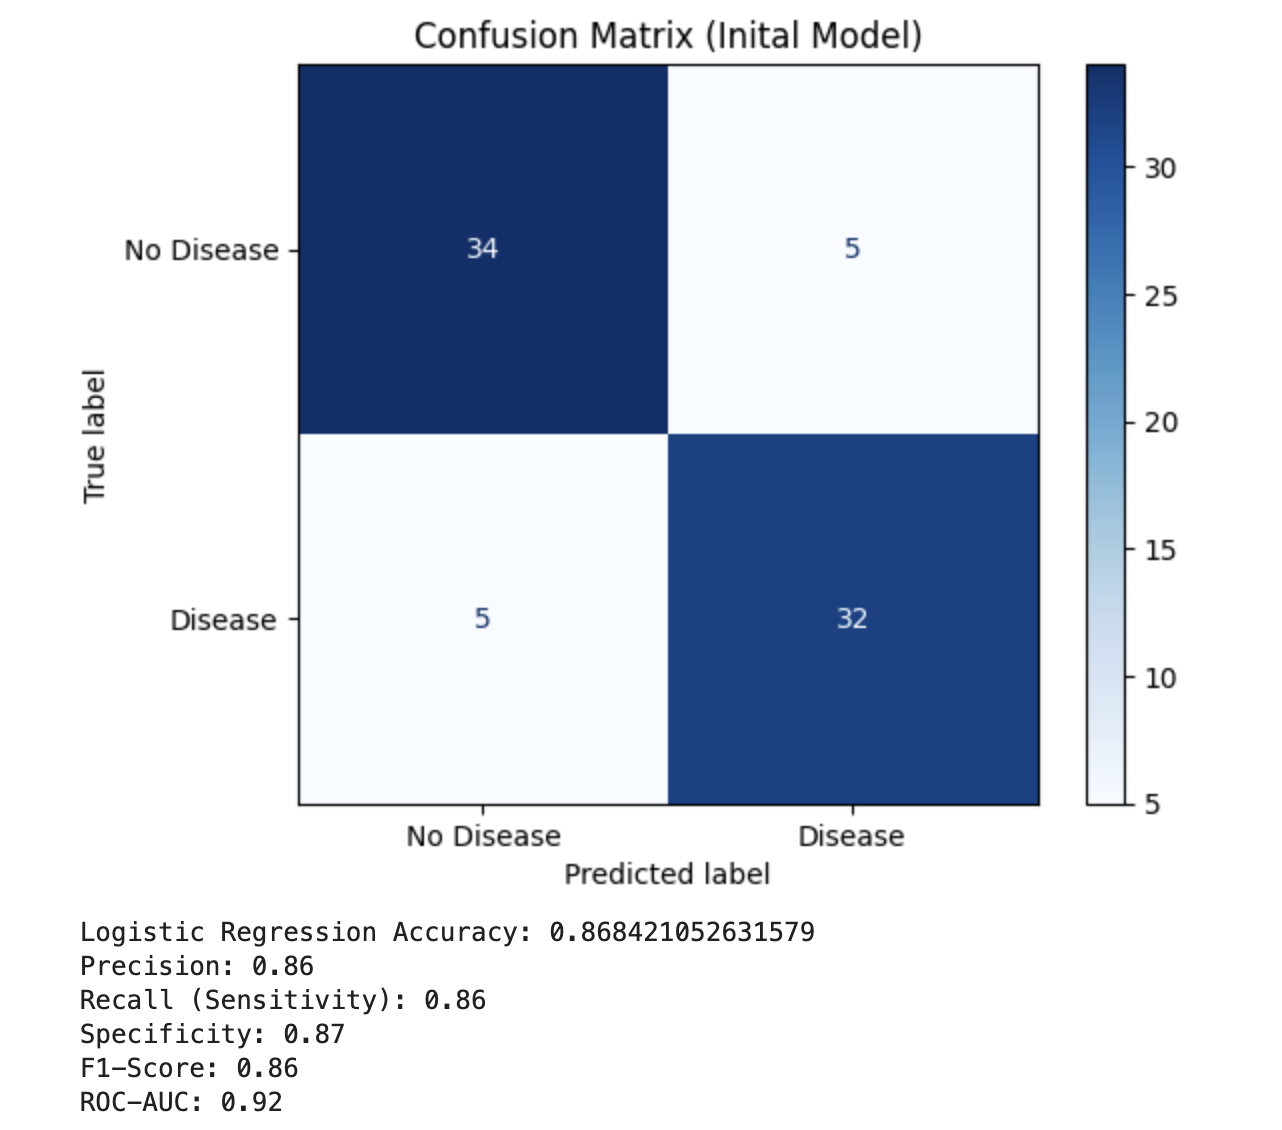
\includegraphics[scale=0.2]{img/confusion_matrix_inital.png}}
    \caption{Initial Logistic Regression Confusion Matrix.}\label{Initial Logistic Regression Confusion Matrix}
\end{figure}

\begin{figure}[htbp]
    \centerline{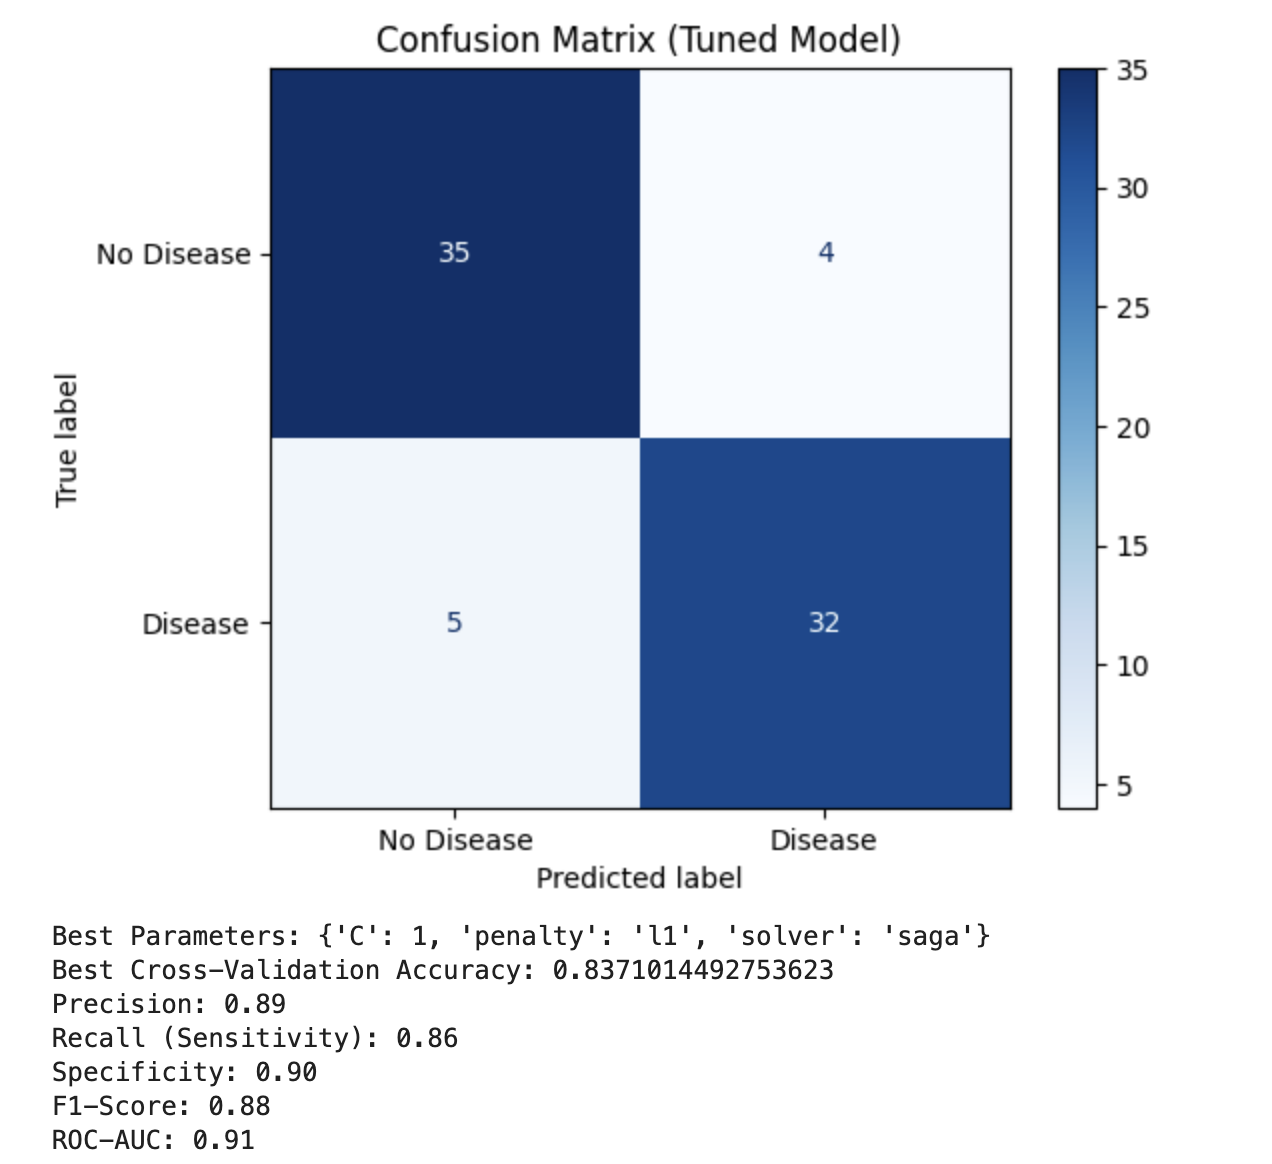
\includegraphics[scale=0.2]{img/confusion_matrix_tuned_model.png}}
    \caption{Tuned Logistic Regression Confusion Matrix.}\label{Tuned Logistic Regression Confusion Matrix}
\end{figure}

The Receiver Operating Characteristic (ROC) curve for the initial model had an AUC value of 0.92, reflecting strong discriminatory capability between classes, while the tuned model achieved a slightly lower AUC of 0.91
By analyzing the confusion matrix and ROC curve, we concluded that the logistic regression model provides robust predictions for detecting heart disease while maintaining low false-positive and false-negative rates. (Fig.~\ref{Initial Logistic Regression Receiver Operating Characteristic (ROC) Curve} \& Fig.~\ref{Tuned Logistic Regression Model Receiver Operating Characteristic (ROC) Curve})

\begin{figure}[htbp]
    \centerline{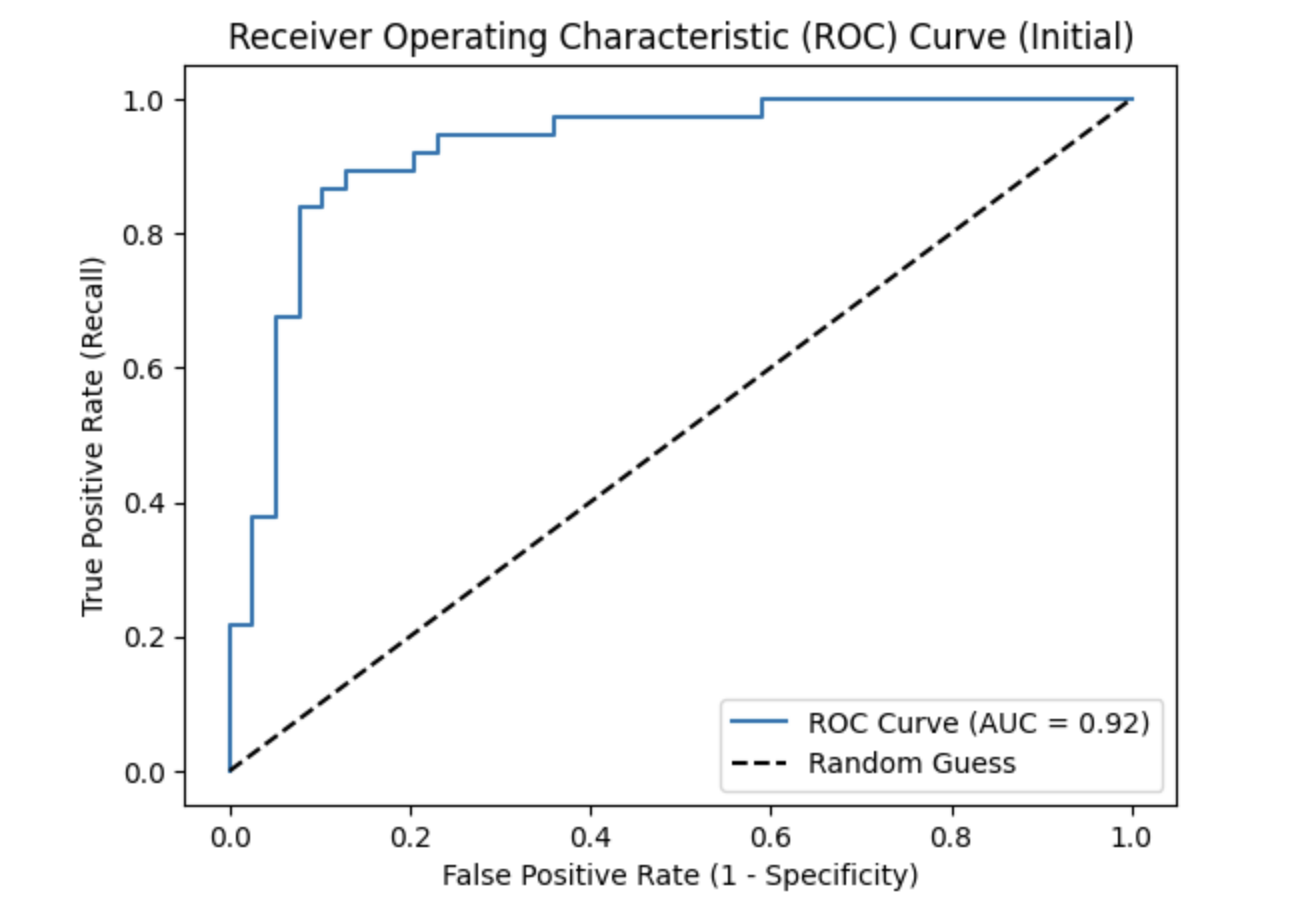
\includegraphics[scale=0.2]{img/receiver_operating_characteristic_curve_inital.png}}
    \caption{Initial Logistic Regression Receiver Operating Characteristic (ROC) Curve.}\label{Initial Logistic Regression Receiver Operating Characteristic (ROC) Curve}
\end{figure}

\begin{figure}[htbp]
    \centerline{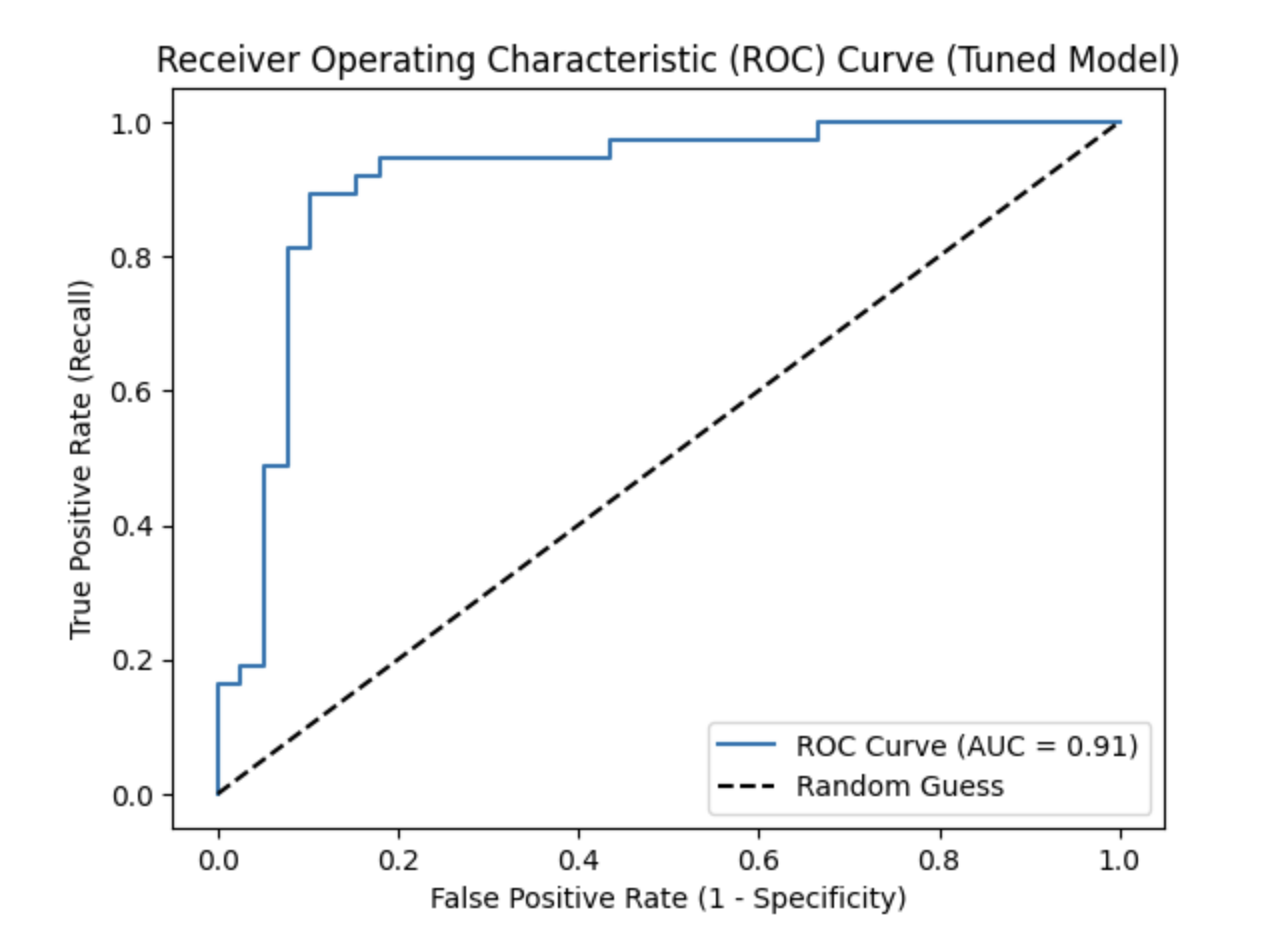
\includegraphics[scale=0.2]{img/receiver_operating_characteristic_curve_tuned_model.png}}
    \caption{Tuned Logistic Regression Model Receiver Operating Characteristic (ROC) Curve.}\label{Tuned Logistic Regression Model Receiver Operating Characteristic (ROC) Curve}
\end{figure}

\subsection{Random Forest}
We developed this model for the prediction of heart disease presence using a Random Forest Classifier. In this regard, we separated numerical and categorical features, imputing their missing values using mean for numerical, most frequent for categorical-followed by the application of standard scaling and one-hot encoding. Data preprocessed was passed to a pipeline that integrates the Random Forest Classifier.

Then we did some hyperparameter tuning, however the results were a bit worse than using the default parameters and cross-validation. Therefore, for the evaluation, we used cross-validation. Metrics used to assess the effectiveness of this model include precision, recall, F1-score, specificity, and a confusion matrix. (Fig.~\ref{Tuned Random Forest Precision Recall Curve} \& Fig.~\ref{Tuned Random Forest Confusion Matrix})

\begin{figure}[htbp]
    \centerline{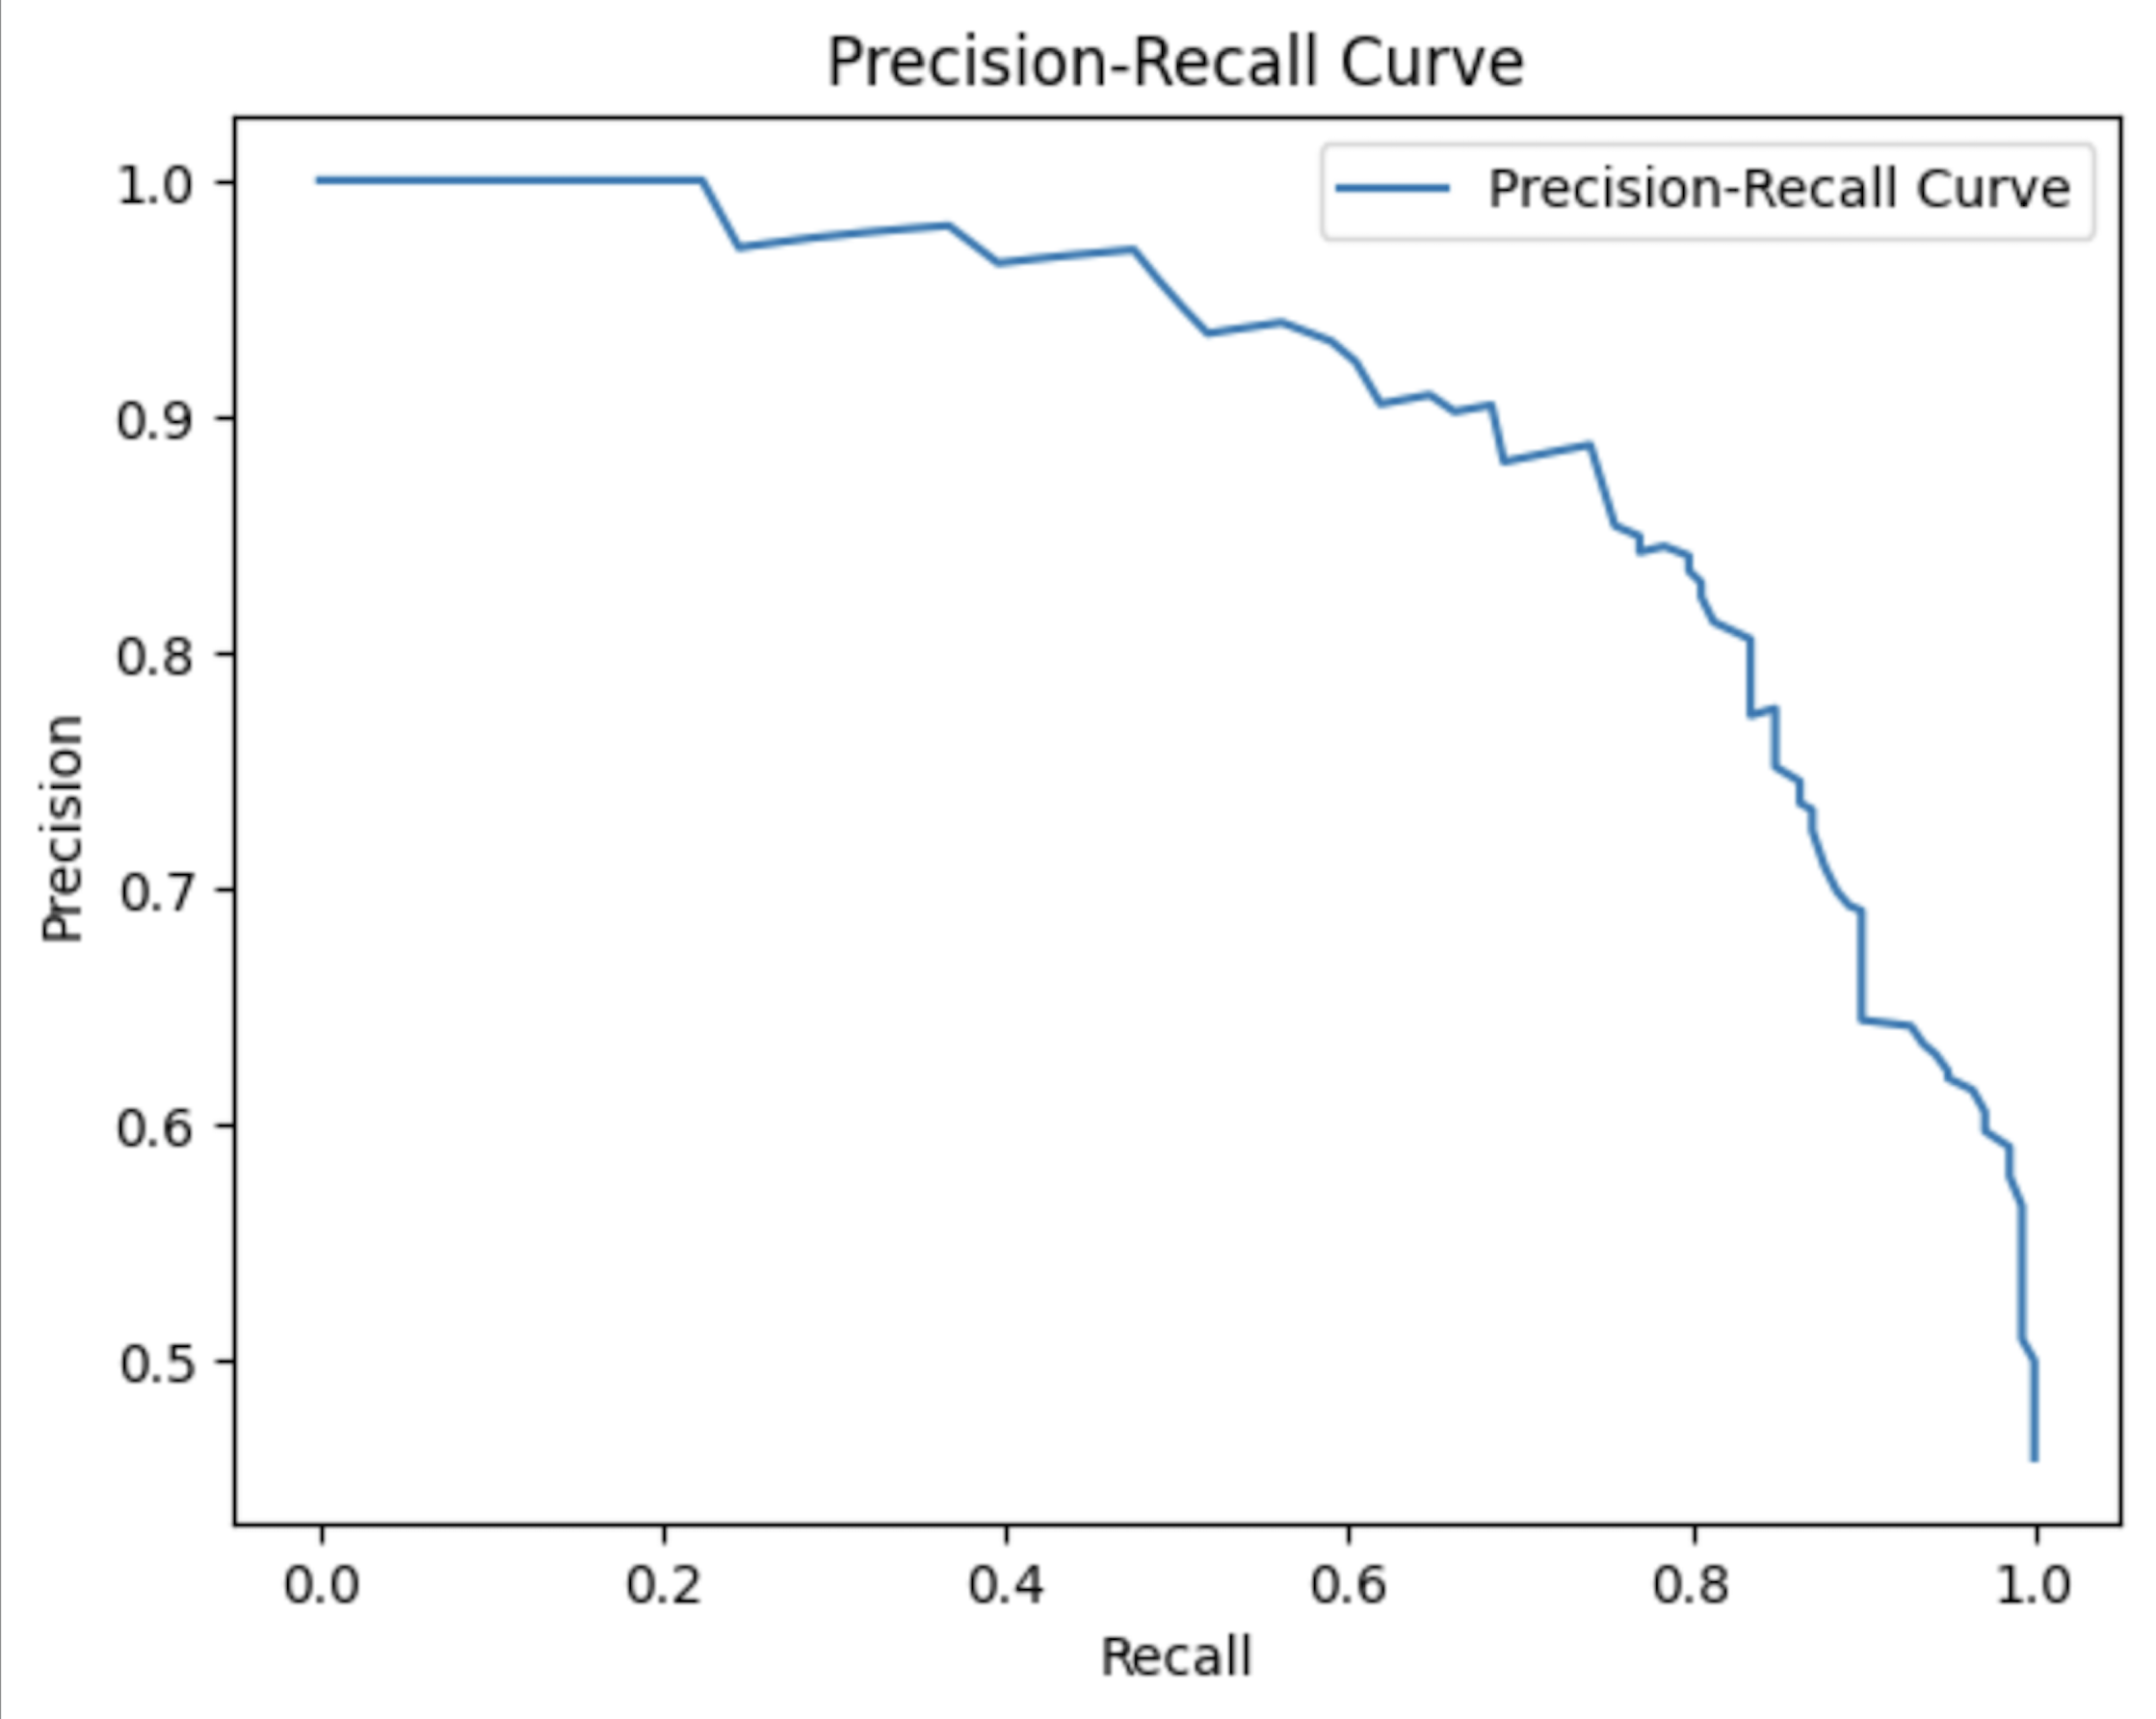
\includegraphics[scale=0.2]{img/random_forest_precision_recall_optimized.png}}
    \caption{Tuned Random Forest Precision Recall Curve.}\label{Tuned Random Forest Precision Recall Curve}
\end{figure}

\begin{figure}[htbp]
    \centerline{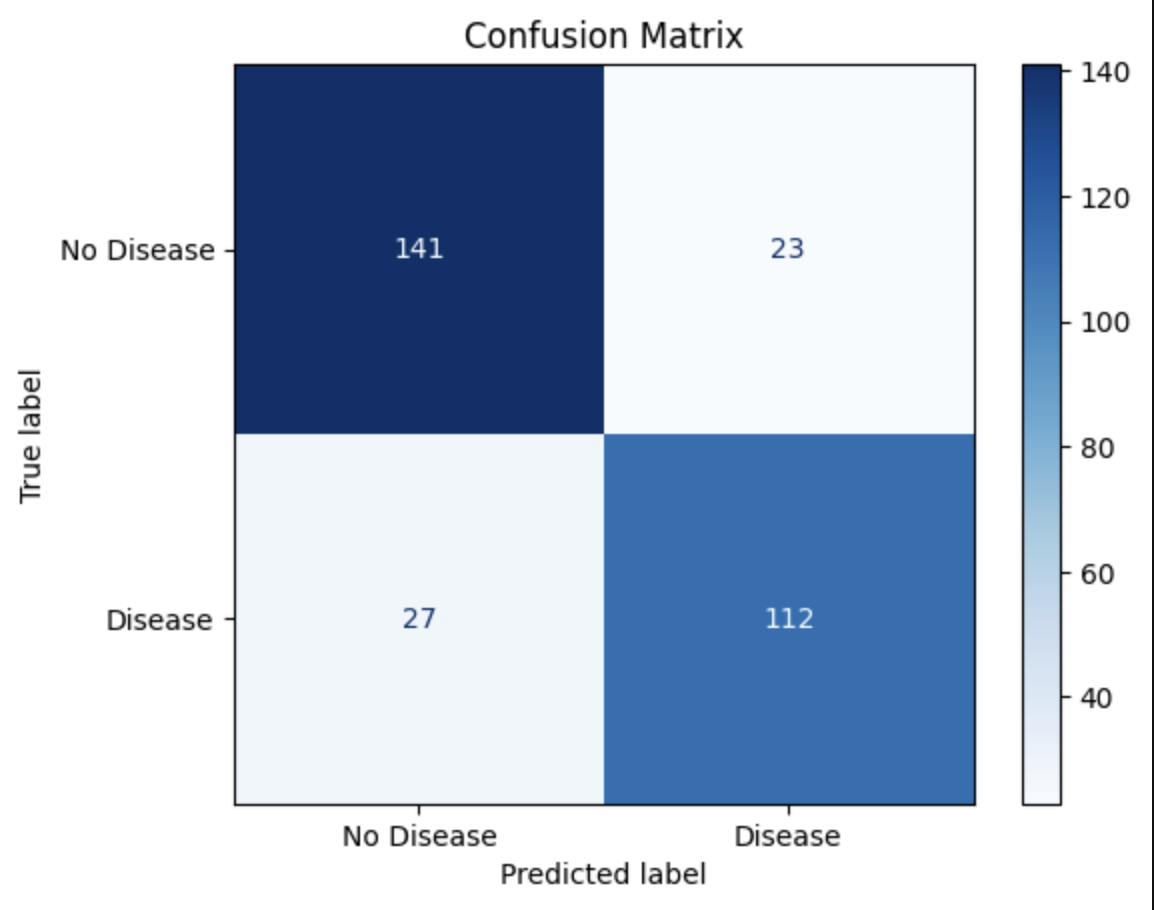
\includegraphics[scale=0.4]{img/random_forest_confusion_matrix_optimized.png}}
    \caption{Tuned Random Forest Confusion Matrix.}\label{Tuned Random Forest Confusion Matrix}
\end{figure}

\subsection{Artificial Neural Network}

To build the artificial neural network (ANN) model, we used the Keras library in Python. We first developed a simple model without hyperparameter tuning or cross-validation using 13 neurons in the input layer for each feature, 64 neurons in the hidden layers, and one output neuron. We used the ReLU activation function for the hidden layers and the sigmoid activation function for the output neuron. We used the binary cross-entropy loss function 
\[
-\frac{1}{n}\sum_{i=1}^{n}y_i \log (P(y_i)) + (1 - y_i) \log (1 - P(y_i))
\]
where \(y_i\) is the true label and \(P(y_i)\) is the predicted probability of the true label.
We used mini-batch gradient descent as the optimization technique. We trained the model for 100 epochs with a batch size of 10. However, when we examined the training and testing loss, we found that the model was greatly overfitting the training data, as seen in Fig.~\ref{annoverfitting}. 

\begin{figure}[htbp]
    % \centerline{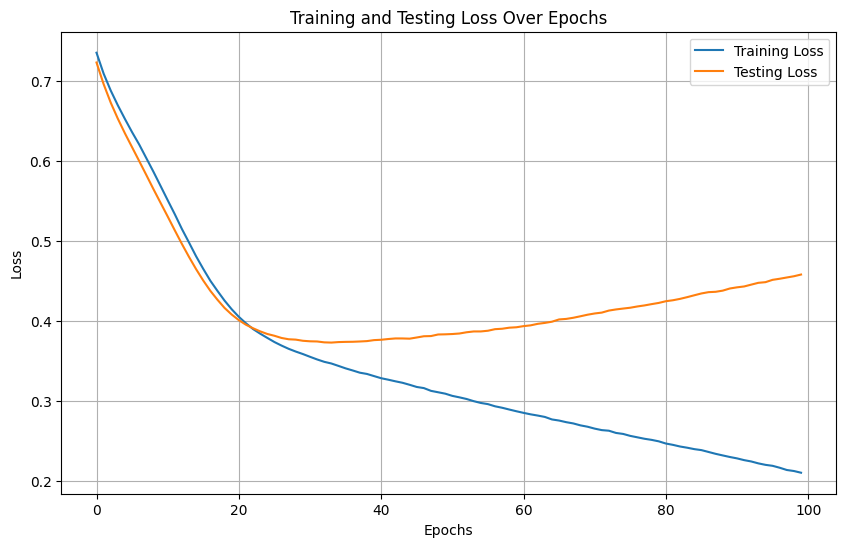
\includegraphics[width=0.7\columnwidth]{img/annoverfitting.png}}
    \centerline{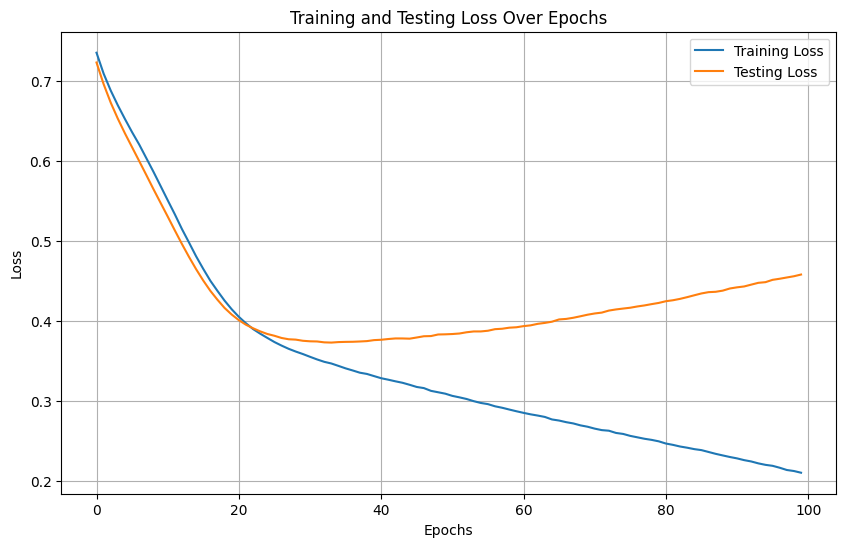
\includegraphics[scale=0.435]{img/annoverfitting.png}}
    \caption{Initial ANN model Training and Testing Loss.}\label{annoverfitting}
\end{figure}

To address this issue, we added 5-fold cross-validation and hyperparameter tuning, with dropout and momentum added. We used the GridSearchCV function from the scikit-learn library to perform a grid search over different values for the number of hidden layers (1, 2, 3), the number of neurons in each hidden layer (32, 64, 128), the dropout rate (0.1, 0.3) and the momentum term (0.5, 0.9). To further prevent overfitting and to reduce computation time, we reduced the number of epochs the model was trained for from 100 to 50. We found that the best model had three hidden layers with 128 neurons each, with a dropout rate of 0.3 and momentum term of 0.5. The best model achieved an accuracy of 0.91 on the test set, which was a significant improvement over the simple model which had an accuracy of 0.85. The confusion matrix for the best model is shown in Fig.~\ref{annconfusion}.

\begin{figure}[htbp]
    % \centerline{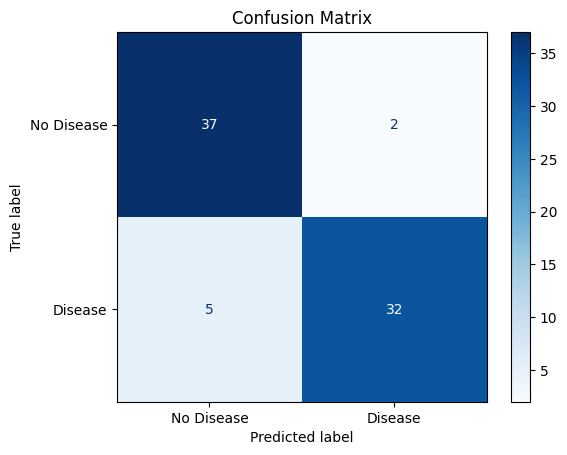
\includegraphics[width=0.7\columnwidth]{img/annconfusion.png}}
    \centerline{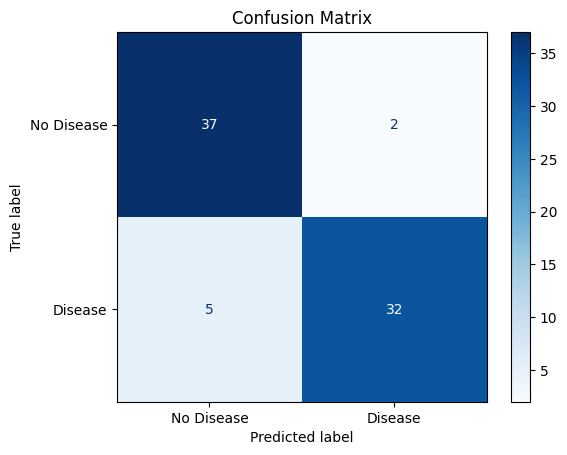
\includegraphics[scale=.65]{img/annconfusion.png}}
    \caption{Tuned ANN model Confusion matrix.}\label{annconfusion}
\end{figure}

\subsection{Model Comparison}
The ANN was a complex model to capture nonlinear patterns and interactions in the data-a high-performance option for intricate relationships that might be missed by simpler models. The Random Forest model makes robust predictions on tabular data by effectively handling feature interactions and nonlinear relationships, while also providing insight into feature importance for better understanding of the dataset. Logistic Regression was the baseline model that provided a point of reference with which other results could be compared due to its transparency and interpretability, mainly when the features were related linearly to the target variable in our dataset.

Artificial Neural Networks (ANN) had superior prediction performance compared to the other three models. Its ability to simulate intricate patterns and relationships among characteristics made it especially adept at capturing the subtleties of the Cleveland dataset. Methods like hyperparameter tuning and dropout improved the model's performance, yielding more accuracy than Logistic Regression and Random Forest. Although ANN required more computer resources for training, it adeptly used the dataset's complexity to get exceptional outcomes. This accuracy makes ANN an attractive option for critical applications where precision is essential.

The selection of the best appropriate model is contingent upon the particular needs of the application. Logistic Regression is optimal for situations emphasizing simplicity and interpretability, but Random Forest offers a resilient compromise for managing complexity. Artificial Neural Networks (ANN) are the optimal selection for attaining superior predicted accuracy, particularly in scenarios where precision is paramount. This comparison emphasizes the need of customizing machine learning models to meet the specific requirements of healthcare data, balancing performance, interpretability, and computational efficiency to guarantee their practical use in medical diagnostics.